%% bare_jrnl.tex
%% V1.3
%% 2007/01/11
%% by Michael Shell
%% see http://www.michaelshell.org/
%% for current contact information.
%%
%% This is a skeleton file demonstrating the use of IEEEtran.cls
%% (requires IEEEtran.cls version 1.7 or later) with an IEEE journal paper.
%%
%% Support sites:
%% http://www.michaelshell.org/tex/ieeetran/
%% http://www.ctan.org/tex-archive/macros/latex/contrib/IEEEtran/
%% and
%% http://www.ieee.org/



% *** Authors should verify (and, if needed, correct) their LaTeX system  ***
% *** with the testflow diagnostic prior to trusting their LaTeX platform ***
% *** with production work. IEEE's font choices can trigger bugs that do  ***
% *** not appear when using other class files.                            ***
% The testflow support page is at:
% http://www.michaelshell.org/tex/testflow/


%%*************************************************************************
%% Legal Notice:
%% This code is offered as-is without any warranty either expressed or
%% implied; without even the implied warranty of MERCHANTABILITY or
%% FITNESS FOR A PARTICULAR PURPOSE! 
%% User assumes all risk.
%% In no event shall IEEE or any contributor to this code be liable for
%% any damages or losses, including, but not limited to, incidental,
%% consequential, or any other damages, resulting from the use or misuse
%% of any information contained here.
%%
%% All comments are the opinions of their respective authors and are not
%% necessarily endorsed by the IEEE.
%%
%% This work is distributed under the LaTeX Project Public License (LPPL)
%% ( http://www.latex-project.org/ ) version 1.3, and may be freely used,
%% distributed and modified. A copy of the LPPL, version 1.3, is included
%% in the base LaTeX documentation of all distributions of LaTeX released
%% 2003/12/01 or later.
%% Retain all contribution notices and credits.
%% ** Modified files should be clearly indicated as such, including  **
%% ** renaming them and changing author support contact information. **
%%
%% File list of work: IEEEtran.cls, IEEEtran_HOWTO.pdf, bare_adv.tex,
%%                    bare_conf.tex, bare_jrnl.tex, bare_jrnl_compsoc.tex
%%*************************************************************************

% Note that the a4paper option is mainly intended so that authors in
% countries using A4 can easily print to A4 and see how their papers will
% look in print - the typesetting of the document will not typically be
% affected with changes in paper size (but the bottom and side margins will).
% Use the testflow package mentioned above to verify correct handling of
% both paper sizes by the user's LaTeX system.
%
% Also note that the "draftcls" or "draftclsnofoot", not "draft", option
% should be used if it is desired that the figures are to be displayed in
% draft mode.
%
\documentclass[journal]{IEEEtran}
%
% If IEEEtran.cls has not been installed into the LaTeX system files,
% manually specify the path to it like:
% \documentclass[journal]{../sty/IEEEtran}





% Some very useful LaTeX packages include:
% (uncomment the ones you want to load)


% *** MISC UTILITY PACKAGES ***
%
%\usepackage{ifpdf}
% Heiko Oberdiek's ifpdf.sty is very useful if you need conditional
% compilation based on whether the output is pdf or dvi.
% usage:
% \ifpdf
%   % pdf code
% \else
%   % dvi code
% \fi
% The latest version of ifpdf.sty can be obtained from:
% http://www.ctan.org/tex-archive/macros/latex/contrib/oberdiek/
% Also, note that IEEEtran.cls V1.7 and later provides a builtin
% \ifCLASSINFOpdf conditional that works the same way.
% When switching from latex to pdflatex and vice-versa, the compiler may
% have to be run twice to clear warning/error messages.





\usepackage{comment}
\usepackage{array}

% *** CITATION PACKAGES ***
%
%\usepackage{natbib}
\usepackage{cite}
%\usepackage{subcaption}
% cite.sty was written by Donald Arseneau
% V1.6 and later of IEEEtran pre-defines the format of the cite.sty package
% \cite{} output to follow that of IEEE. Loading the cite package will
% result in citation numbers being automatically sorted and properly
% "compressed/ranged". e.g., [1], [9], [2], [7], [5], [6] without using
% cite.sty will become [1], [2], [5]--[7], [9] using cite.sty. cite.sty's
% \cite will automatically add leading space, if needed. Use cite.sty's
% noadjust option (cite.sty V3.8 and later) if you want to turn this off.
% cite.sty is already installed on most LaTeX systems. Be sure and use
% version 4.0 (2003-05-27) and later if using hyperref.sty. cite.sty does
% not currently provide for hyperlinked citations.
% The latest version can be obtained at:
% http://www.ctan.org/tex-archive/macros/latex/contrib/cite/
% The documentation is contained in the cite.sty file itself.






% *** GRAPHICS RELATED PACKAGES ***
%
\ifCLASSINFOpdf
   \usepackage[pdftex]{graphicx}
  % declare the path(s) where your graphic files are
  % \graphicspath{{../pdf/}{../jpeg/}}
  % and their extensions so you won't have to specify these with
  % every instance of \includegraphics
  % \DeclareGraphicsExtensions{.pdf,.jpeg,.png}
\else
  % or other class option (dvipsone, dvipdf, if not using dvips). graphicx
  % will default to the driver specified in the system graphics.cfg if no
  % driver is specified.
   \usepackage[dvips]{graphicx}
  % declare the path(s) where your graphic files are
  % \graphicspath{{../eps/}}
  % and their extensions so you won't have to specify these with
  % every instance of \includegraphics
  % \DeclareGraphicsExtensions{.eps}
\fi
% graphicx was written by David Carlisle and Sebastian Rahtz. It is
% required if you want graphics, photos, etc. graphicx.sty is already
% installed on most LaTeX systems. The latest version and documentation can
% be obtained at: 
% http://www.ctan.org/tex-archive/macros/latex/required/graphics/
% Another good source of documentation is "Using Imported Graphics in
% LaTeX2e" by Keith Reckdahl which can be found as epslatex.ps or
% epslatex.pdf at: http://www.ctan.org/tex-archive/info/
%
% latex, and pdflatex in dvi mode, support graphics in encapsulated
% postscript (.eps) format. pdflatex in pdf mode supports graphics
% in .pdf, .jpeg, .png and .mps (metapost) formats. Users should ensure
% that all non-photo figures use a vector format (.eps, .pdf, .mps) and
% not a bitmapped formats (.jpeg, .png). IEEE frowns on bitmapped formats
% which can result in "jaggedy"/blurry rendering of lines and letters as
% well as large increases in file sizes.
%
% You can find documentation about the pdfTeX application at:
% http://www.tug.org/applications/pdftex



\usepackage{tikz}
\usetikzlibrary{arrows.meta,shapes,shadows,arrows,decorations.pathreplacing,decorations.markings}
\usepackage{longtable}
\usepackage{tabularx}
\usepackage{multicol}
% *** MATH PACKAGES ***
%
\usepackage[cmex10]{amsmath}
% A popular package from the American Mathematical Society that provides
% many useful and powerful commands for dealing with mathematics. If using
% it, be sure to load this package with the cmex10 option to ensure that
% only type 1 fonts will utilized at all point sizes. Without this option,
% it is possible that some math symbols, particularly those within
% footnotes, will be rendered in bitmap form which will result in a
% document that can not be IEEE Xplore compliant!
%
% Also, note that the amsmath package sets \interdisplaylinepenalty to 10000
% thus preventing page breaks from occurring within multiline equations. Use:
%\interdisplaylinepenalty=2500
% after loading amsmath to restore such page breaks as IEEEtran.cls normally
% does. amsmath.sty is already installed on most LaTeX systems. The latest
% version and documentation can be obtained at:
% http://www.ctan.org/tex-archive/macros/latex/required/amslatex/math/





% *** SPECIALIZED LIST PACKAGES ***
%
%\usepackage{algorithmic}
% algorithmic.sty was written by Peter Williams and Rogerio Brito.
% This package provides an algorithmic environment fo describing algorithms.
% You can use the algorithmic environment in-text or within a figure
% environment to provide for a floating algorithm. Do NOT use the algorithm
% floating environment provided by algorithm.sty (by the same authors) or
% algorithm2e.sty (by Christophe Fiorio) as IEEE does not use dedicated
% algorithm float types and packages that provide these will not provide
% correct IEEE style captions. The latest version and documentation of
% algorithmic.sty can be obtained at:
% http://www.ctan.org/tex-archive/macros/latex/contrib/algorithms/
% There is also a support site at:
% http://algorithms.berlios.de/index.html
% Also of interest may be the (relatively newer and more customizable)
% algorithmicx.sty package by Szasz Janos:
% http://www.ctan.org/tex-archive/macros/latex/contrib/algorithmicx/




% *** ALIGNMENT PACKAGES ***
%
\usepackage{array}
% Frank Mittelbach's and David Carlisle's array.sty patches and improves
% the standard LaTeX2e array and tabular environments to provide better
% appearance and additional user controls. As the default LaTeX2e table
% generation code is lacking to the point of almost being broken with
% respect to the quality of the end results, all users are strongly
% advised to use an enhanced (at the very least that provided by array.sty)
% set of table tools. array.sty is already installed on most systems. The
% latest version and documentation can be obtained at:
% http://www.ctan.org/tex-archive/macros/latex/required/tools/


%\usepackage{mdwmath}
\usepackage{mdwtab}
% Also highly recommended is Mark Wooding's extremely powerful MDW tools,
% especially mdwmath.sty and mdwtab.sty which are used to format equations
% and tables, respectively. The MDWtools set is already installed on most
% LaTeX systems. The lastest version and documentation is available at:
% http://www.ctan.org/tex-archive/macros/latex/contrib/mdwtools/


% IEEEtran contains the IEEEeqnarray family of commands that can be used to
% generate multiline equations as well as matrices, tables, etc., of high
% quality.


\usepackage{eqparbox}
% Also of notable interest is Scott Pakin's eqparbox package for creating
% (automatically sized) equal width boxes - aka "natural width parboxes".
% Available at:
% http://www.ctan.org/tex-archive/macros/latex/contrib/eqparbox/





% *** SUBFIGURE PACKAGES ***
\usepackage[tight,footnotesize]{subfigure}
% subfigure.sty was written by Steven Douglas Cochran. This package makes it
% easy to put subfigures in your figures. e.g., "Figure 1a and 1b". For IEEE
% work, it is a good idea to load it with the tight package option to reduce
% the amount of white space around the subfigures. subfigure.sty is already
% installed on most LaTeX systems. The latest version and documentation can
% be obtained at:
% http://www.ctan.org/tex-archive/obsolete/macros/latex/contrib/subfigure/
% subfigure.sty has been superceeded by subfig.sty.



%\usepackage[caption=false]{caption}
%\usepackage[font=footnotesize]{subfig}
% subfig.sty, also written by Steven Douglas Cochran, is the modern
% replacement for subfigure.sty. However, subfig.sty requires and
% automatically loads Axel Sommerfeldt's caption.sty which will override
% IEEEtran.cls handling of captions and this will result in nonIEEE style
% figure/table captions. To prevent this problem, be sure and preload
% caption.sty with its "caption=false" package option. This is will preserve
% IEEEtran.cls handing of captions. Version 1.3 (2005/06/28) and later 
% (recommended due to many improvements over 1.2) of subfig.sty supports
% the caption=false option directly:
%\usepackage[caption=false,font=footnotesize]{subfig}
%
% The latest version and documentation can be obtained at:
% http://www.ctan.org/tex-archive/macros/latex/contrib/subfig/
% The latest version and documentation of caption.sty can be obtained at:
% http://www.ctan.org/tex-archive/macros/latex/contrib/caption/




% *** FLOAT PACKAGES ***
%
%\usepackage{fixltx2e}
% fixltx2e, the successor to the earlier fix2col.sty, was written by
% Frank Mittelbach and David Carlisle. This package corrects a few problems
% in the LaTeX2e kernel, the most notable of which is that in current
% LaTeX2e releases, the ordering of single and double column floats is not
% guaranteed to be preserved. Thus, an unpatched LaTeX2e can allow a
% single column figure to be placed prior to an earlier double column
% figure. The latest version and documentation can be found at:
% http://www.ctan.org/tex-archive/macros/latex/base/



\usepackage{stfloats}
% stfloats.sty was written by Sigitas Tolusis. This package gives LaTeX2e
% the ability to do double column floats at the bottom of the page as well
% as the top. (e.g., "\begin{figure*}[!b]" is not normally possible in
% LaTeX2e). It also provides a command:
%\fnbelowfloat
% to enable the placement of footnotes below bottom floats (the standard
% LaTeX2e kernel puts them above bottom floats). This is an invasive package
% which rewrites many portions of the LaTeX2e float routines. It may not work
% with other packages that modify the LaTeX2e float routines. The latest
% version and documentation can be obtained at:
% http://www.ctan.org/tex-archive/macros/latex/contrib/sttools/
% Documentation is contained in the stfloats.sty comments as well as in the
% presfull.pdf file. Do not use the stfloats baselinefloat ability as IEEE
% does not allow \baselineskip to stretch. Authors submitting work to the
% IEEE should note that IEEE rarely uses double column equations and
% that authors should try to avoid such use. Do not be tempted to use the
% cuted.sty or midfloat.sty packages (also by Sigitas Tolusis) as IEEE does
% not format its papers in such ways.


%\ifCLASSOPTIONcaptionsoff
%  \usepackage[nomarkers]{endfloat}
% \let\MYoriglatexcaption\caption
% \renewcommand{\caption}[2][\relax]{\MYoriglatexcaption[#2]{#2}}
%\fi
% endfloat.sty was written by James Darrell McCauley and Jeff Goldberg.
% This package may be useful when used in conjunction with IEEEtran.cls'
% captionsoff option. Some IEEE journals/societies require that submissions
% have lists of figures/tables at the end of the paper and that
% figures/tables without any captions are placed on a page by themselves at
% the end of the document. If needed, the draftcls IEEEtran class option or
% \CLASSINPUTbaselinestretch interface can be used to increase the line
% spacing as well. Be sure and use the nomarkers option of endfloat to
% prevent endfloat from "marking" where the figures would have been placed
% in the text. The two hack lines of code above are a slight modification of
% that suggested by in the endfloat docs (section 8.3.1) to ensure that
% the full captions always appear in the list of figures/tables - even if
% the user used the short optional argument of \caption[]{}.
% IEEE papers do not typically make use of \caption[]'s optional argument,
% so this should not be an issue. A similar trick can be used to disable
% captions of packages such as subfig.sty that lack options to turn off
% the subcaptions:
% For subfig.sty:
% \let\MYorigsubfloat\subfloat
% \renewcommand{\subfloat}[2][\relax]{\MYorigsubfloat[]{#2}}
% For subfigure.sty:
% \let\MYorigsubfigure\subfigure
% \renewcommand{\subfigure}[2][\relax]{\MYorigsubfigure[]{#2}}
% However, the above trick will not work if both optional arguments of
% the \subfloat/subfig command are used. Furthermore, there needs to be a
% description of each subfigure *somewhere* and endfloat does not add
% subfigure captions to its list of figures. Thus, the best approach is to
% avoid the use of subfigure captions (many IEEE journals avoid them anyway)
% and instead reference/explain all the subfigures within the main caption.
% The latest version of endfloat.sty and its documentation can obtained at:
% http://www.ctan.org/tex-archive/macros/latex/contrib/endfloat/
%
% The IEEEtran \ifCLASSOPTIONcaptionsoff conditional can also be used
% later in the document, say, to conditionally put the References on a 
% page by themselves.





% *** PDF, URL AND HYPERLINK PACKAGES ***
%
\usepackage{url}
% url.sty was written by Donald Arseneau. It provides better support for
% handling and breaking URLs. url.sty is already installed on most LaTeX
% systems. The latest version can be obtained at:
% http://www.ctan.org/tex-archive/macros/latex/contrib/misc/
% Read the url.sty source comments for usage information. Basically,
% \url{my_url_here}.





% *** Do not adjust lengths that control margins, column widths, etc. ***
% *** Do not use packages that alter fonts (such as pslatex).         ***
% There should be no need to do such things with IEEEtran.cls V1.6 and later.
% (Unless specifically asked to do so by the journal or conference you plan
% to submit to, of course. )


% correct bad hyphenation here
\hyphenation{op-tical net-works semi-conduc-tor}

\pagestyle{empty}
\usepackage{amsmath}
\usepackage{mdwtab}
\usepackage{multirow}
% \usepackage[pdftex]{graphicx}
%\usetikzlibrary{matrix,shapes,arrows,positioning,chains}
\usetikzlibrary{shapes,arrows}
\begin{document}
%
% paper title
% can use linebreaks \\ within to get better formatting as desired
\title{THEORITICAL PREDICTION AND MATHEMATICAL FORMUALTION OF THE MATERIAL  COMPOSITION FOR MICROWAVE ABSORPTION APPLICATIONS}
%
%
% author names and IEEE memberships
% note positions of commas and nonbreaking spaces ( ~ ) LaTeX will not break
% a structure at a ~ so this keeps an author's name from being broken across
% two lines.
% use \thanks{} to gain access to the first footnote area
% a separate \thanks must be used for each paragraph as LaTeX2e's \thanks
% was not built to handle multiple paragraphs
%

\author{Aayushi Arya,Dr GVV Sharma}
%,~\IEEEmembership{Member,~IEEE,}
 %      John~Doe,~\IEEEmembership{Fellow,~OSA,}
  %    and~Jane~Doe,~\IEEEmembership{Life~Fellow,~IEEE}% <-this % stops a space
%  \author{AayushiArya}
%\thanks{M. Shell is with the Department
%of Electrical and Computer Engineering, Georgia Institute of Technology, Atlanta,
%GA, 30332 USA e-mail: (see http://www.michaelshell.org/contact.html).}% <-this % stops a space
%\thanks{J. Doe and J. Doe are with Anonymous University.}% <-this % stops a space
%\thanks{Manuscript received April 19, 2005; revised January 11, 2007.}}

% note the % following the last \IEEEmembership and also \thanks - 
% these prevent an unwanted space from occurring between the last author name
% and the end of the author line. i.e., if you had this:
% 
% \author{....lastname \thanks{...} \thanks{...} }
%                     ^------------^------------^----Do not want these spaces!
%
% a space would be appended to the last name and could cause every name on that
% line to be shifted left slightly. This is one of those "LaTeX things". For
% instance, "\textbf{A} \textbf{B}" will typeset as "A B" not "AB". To get
% "AB" then you have to do: "\textbf{A}\textbf{B}"
% \thanks is no different in this regard, so shield the last } of each \thanks
% that ends a line with a % and do not let a space in before the next \thanks.
% Spaces after \IEEEmembership other than the last one are OK (and needed) as
% you are supposed to have spaces between the names. For what it is worth,
% this is a minor point as most people would not even notice if the said evil
% space somehow managed to creep in.



% The paper headers
\markboth{Journal of \LaTeX\ Class Files,~Vol.~6, No.~1, January~2007}%
{Shell \MakeLowercase{\textit{et al.}}: Bare Demo of IEEEtran.cls for Journals}
% The only time the second header will appear is for the odd numbered pages
% after the title page when using the twoside option.
% 
% *** Note that you probably will NOT want to include the author's ***
% *** name in the headers of peer review papers.                   ***
% You can use \ifCLASSOPTIONpeerreview for conditional compilation here if
% you desire.




% If you want to put a publisher's ID mark on the page you can do it like
% this:
%\IEEEpubid{0000--0000/00\$00.00~\copyright~2007 IEEE}
% Remember, if you use this you must call \IEEEpubidadjcol in the second
% column for its text to clear the IEEEpubid mark.



% use for special paper notices
%\IEEEspecialpapernotice{(Invited Paper)}



\maketitle
\thispagestyle{empty}


\begin{abstract}
%\boldmath
Microwave Absorbers has become an essential requirement in various fields including industrial uses like Radar, Stealth , commercial uses in mobile networking , EMI , EMC, electronic toll collection, social applications like in hospitals , schools , where the microwave flux has crossed the threshold. In the past few years, there has been  an intense experimental work to explore various materials for the different applications , focusssing on their effectiveness, stability. The hit and trial cycles of the experimentation can be reduced with a theoritical model predicting the suitability of material for MA applications, allowing more accurate , rigorous and wide prespective for the experimentation. Thus, in this work , an attempt has been made provide a conceptual and theoritical mathematical formulation based model to predict the suitability of various elements and their composition for specified application. The model is based on Transmission Line Theory, Polarizability, dielectric response of material. The  parameters are derived for the MA  are characteristic impedance, input impedance , permittivity , permeability polarizability , Molar refraction ratio, Polarisation Energy. Using the above paramters and the material properties like its global hardness factor, we conclude to a set of theoritical atomic radii , which can be suitable for the absorption at the specified frequency , which is 2.54 GHz ( ISM band -immensely used in various eelctronic applications). Further a composition of two or more elements viz. oxides of material, alloys , and multi cation oxides, can be predicted by comparing their spatial energy parameter , which depends on their individual valency and global hardness factor.This work is beneficial for not only understanding the fundamental molecular level perspective of the absorbers but also in providing a conceptual and engineering aspect to further explore new materials for the microwave absorption , with less error rate.
\end{abstract}
% IEEEtran.cls defaults to using nonbold math in the Abstract.
% This preserves the distinction between vectors and scalars. However,
% if the journal you are submitting to favors bold math in the abstract,
% then you can use LaTeX's standard command \boldmath at the very start
% of the abstract to achieve this. Many IEEE journals frown on math
% in the abstract anyway.

% Note that keywords are not normally used for peerreview papers.
\begin{IEEEkeywords}
EMI , Reflection Loss, Resonance, Dielectric Parameters,Polarisation Energy,Atomic Radii.
\end{IEEEkeywords}






% For peer review papers, you can put extra information on the cover
% page as needed:
% \ifCLASSOPTIONpeerreview
% \begin{center} \bfseries EDICS Category: 3-BBND \end{center}
% \fi
%
% For peerreview papers, this IEEEtran command inserts a page break and
% creates the second title. It will be ignored for other modes.
\IEEEpeerreviewmaketitle



\section{Introduction}
% The very first letter is a 2 line initial drop letter followed
% by the rest of the first word in caps.
% 
% form to use if the first word consists of a single letter:
% \IEEEPARstart{A}{demo} file is ....
% 
% form to use if you need the single drop letter followed by
% normal text (unknown if ever used by IEEE):
% \IEEEPARstart{A}{}demo file is ....
% 
% Some journals put the first two words in caps:
% \IEEEPARstart{T}{his demo} file is ....
% 
% Here we have the typical use of a "T" for an initial drop letter
% and "HIS" in caps to complete the first word.
\IEEEPARstart{M}{icrowave Absorbers} , has now become an area of  immense research for both electronic field and materials design . The immediate need of Microwave absorbers is highlighted due to their necessity in the current technological scenario. need Due to the exponential growth of the usage of high frequency  electronic hardware and wireless communication, there is a dramatical increase of the microwaves flux in the ambient surroundings , which causes ElectroMagnetic Interference amomg the underlying circuits undesirably by generating unwanted noise, cross connection ,false output etc. The critical exposure of microwaves  also has harmful effects on the health , especially for hospitals, schools and highly populated residential areas. This creates a  need to mitigate the surrounding EM wave  noise, has driven researchers to develop materials that can effectively absorb the unwanted radiations ,protecting the underneath circuitry. Various materials and their composition are investigated using experimental procedures like Vector Network Analyzer, Impedance Analyzer to test their ability as absorbers. Meanwhile , there is also ongoing work to theoritically understand and model Microwave Absorbers. There are range of wave theory based electrical, magnetic parameters associated with the working of MA.
First is the Reflection Loss and the Characteristic Impedance of a Microwave absorber that can be calculated using Transmission Line Theory \cite{YingL2}.The latter is an intrinsic property independent of the thickness of the sample.
Similar theory is applicable to ferrite based microwave absorbers conatining both electric and magnetic dipoles represnted by  permittivity and permeability respectively \cite{YingL}.The oscillations of dipoles in a MA are both resonant and non resonant. . A detailed absorption model is then provided to include all the above elements in the basics of absorption formulas of transmission line theory.

There has been also works to correlate the electrical/magnetic parameter and physical parameters of microwave absorbers. Analyising polarizability gives an insight into the wave absorbing power of a material. Following this , in \cite{Erbium} , the Lorentz-Lorenz equation was used to estimate  the electronic polarizability of ions in oxide glasses , based on their refractive indices and band gap energy.In \cite{dimitrov1999effect} , the author further discusses an Interaction Parameter for oxides based  on the polarizability of oxide ion, dtermined from the refractive index. This Parameter is used as a measure of the interionic interaction between cations and anions created due to the charge overlap of the outermost electronic orbitals.The charge overlap and the polarizability of cation and anions both affect the Interaction Parameter. This Parameter serves as an index to estimate the optical  properties of oxide glasses. Siimilarly for magnetic based microwave absorbers the magnetic dipole moment can be used as a measure for microwave absprtion.  This consecutive dependency of  properties when modelled mathematically using energy parmeter can provide a useful tool for prediction of new compositions based suitable microwave absorbing materials. The energy parameter when normalized can be directly related to the atomic radii \cite{korablev2018calculations}.
In this paper, an attempt has been made to theoritically derive the parameter related to a microwave absorber. First the transmission line theory was used to determine the electrical parameters including characteristic impedance, reflection loss, permittivity and permeability, resonance frequency . From the above paremters and a set of equations expalined below we derived  the physical parameters like polarizability, dipolar frequency . spatial energy parameter . From this we derived   the atomic range of suitable atomic radii . The compositions can be predicted by comparing the effective Energy Parameter. This approach covers all the necessary  properties required for a microwave absorber. It can be beneficial in filling the gap between the molecular and the physical properties of an absorber . It can help in predicting new compositions for efficient microwave absorbption.
\newline
\subsection{Description of Theoritical Calculation}




%\resizebox{0.5\textwidth}{!}{
	%	\begin{table}
\begin{flushleft}
	

\begin{figure}
\resizebox{0.5\textwidth}{!}{
	
		


	\begin{tabular}{|c|c|c|c|}
		\hline 
		Constant & \multicolumn{2}{|l|}{Description} & Value \\ 
		\hline
		R.L & \multicolumn{2}{|l|}{Reflection Loss} &-20 dB \\
		\hline
		
		${Z_{o}}_{free}$ & \multicolumn{2}{|l|}{Characteristic Impedance of Free Space} & 377 $\Omega$ \\
		\hline
		$f_r$ & \multicolumn{2}{|l|}{Resonance Frequency} & 2.54GHz \\
		\hline
		$\zeta$ &\multicolumn{2}{|l|}{ Damping Factor} & 1.5 \\
		\hline
		$\triangle f_r$ & \multicolumn{2}{|l|}{Bandwidth} & 7.7 GHz \\
		\hline
		$\omega_r$ & \multicolumn{2}{|l|}{angular resonance frequency} & $ 1.53x10^{10} rad/sec$ \\
		\hline
		$\omega_r$ & \multicolumn{2}{|l|}{angular bandwidth } & $ 4.83x10^{10} rad/sec$ \\
		\hline
		$\omega$ &\multicolumn{2}{|l|}{ Upper frequency limit}  & $5 x 10^{10} rad/sec$ \\
		\hline
		A &\multirow{3}{*}{ Cauchy  dispersion}  & $A = 1+ {n_o}^2$ ,
		$n_o $ \tiny{=upper limit of refractive index }& 4.41\\
		\cline{1-1} \cline{3-4}
		B              &             &      $B = (2 \pi c)^2 \dfrac{\chi_e(0)}{{\omega_{oe}}^2}$     ,   $ {\omega_{oe}}^2 = \dfrac{{\omega_o}^2}{{n_o}^2}$    &      \\
		\cline{1-1} \cline{3-4}
		C              &              &    $C= \dfrac{B}{2 A^{1/2}}$              & $3.32x10^{-3}$       \\
		\cline{1-1} \cline{3-4}
		\hline
		$\mu_B$ & \multicolumn{2}{|l|}{Bohr Magneton } & $9.27 X 10^{-21} erg/ gauss$ (CGS unit) \\
		\hline
		$\mu_o$ &  \multicolumn{2}{|l|}{Free Space Permeability} &  $4 \pi X 10^{-7} Hm^{-1}$ \\
		\hline
		$\epsilon_o$ & \multicolumn{2}{|l|}{Free Space Permittivity} & $8.85 X 10^{-12} F m^{-1}$ \\
		\hline
		T & \multicolumn{2}{|l|}{ Absolute Temperature} & 300 K \\
		\hline
		m & \multicolumn{2}{|l|}{ Mass of electron} & $9.1 X 10 ^{-31} Kg $ \\
		\hline
		$k_B$ & \multicolumn{2}{|l|}{Boltzmann Constant } & $1.38 X 10 ^{-23} J.K^{-1}$ \\
		\hline
		N & \multicolumn{2}{|l|}{Avagadro Number } & $6.022 X 10 ^{23}$ \\
		\hline
		$q^2 /2 $ & \multicolumn{2}{|l|}{ratio of unit charge to energy in C.G.S unit} & $7.19 X 10^{-8}$ \\
		\hline
		
	\end{tabular}
	% \end{table}
%}

}
	
	\end{figure}
\end{flushleft}

\onecolumn
\subsection{FLOW-CHART-FOR COMPLETE-CALCULATIONS}
\tikzstyle{decision} = [diamond, draw, fill=blue!20, 
text width=4.5em, text badly centered, node distance=3cm, inner sep=0pt]
\tikzstyle{block} = [rectangle, draw, fill=blue!10, 
text width=5em, text centered, rounded corners, minimum height=4em]
\tikzstyle{line} = [draw, -latex']
\tikzstyle{cloud} = [draw, ellipse,fill=red!20, node distance=3cm,
minimum height=1em,text width=5em]
\begin{center}
	\makebox[0.4\textwidth][c]{\begin{tikzpicture}[scale=2,node distance = 1.5 cm, nodes = {align = center}, >=latex,anchor=center, text width=2em]
		%\makebox[\textwidth][c]{\begin{tikzpicture}[scale=2, auto, every node/.style={font=\footnotesize, >=stealth,node distance=1cm,anchor=base,text width=5em}]
		%node distance = 2 cm , anchor=center]
		%\begin{tikzpicture}
		% Place nodes
		\node [block, align= center] (init) {Microwave Asorber};
		\node [block, below of=init] (Fr) {Resonance frequency fr};
		\node [cloud, left of=Fr, node distance=5.5 cm] (Rl) {Reflection Loss RL};
		\node [cloud, right of=Fr, node distance=5 cm] (delta) {Bandwidth Delta fr};
		\node [block, below of=Rl, node distance=3cm, text width=3cm] (in){\small{Input impedance 
				$ Z_{in} = \dfrac{1+10^{\frac{R.L}{20}}}{1-10^{\frac{R.L}{20}}}$}}; 
		\node [block, below of=in,text width = 2cm,node distance=2cm] (Zo) {{characteristic Impedance
				${Z_o}_{MA} = 4 x Z_{in} x 10^{\frac{R.L}{20}}$}};
		\node [block, left of=Zo, node distance=3 cm] (ratio) {Ratio of permeabilit isto permittivity $Z_in = \sqrt{\frac{\mu_r}{\epsilon_r}}$};
		\node [block, below of=Zo,text width = 3cm, node distance = 3cm] (Pm) { \small{ Min refarctive index $n_1 = \sqrt{\mu_r \epsilon_r} = \dfrac{ c {Z_{in}}_{MA}}{2 \pi f d {Z_{o}}_{MA}} \sqrt{\dfrac{\epsilon_r}{\mu_r}}$}};
		
		
		\node [block, left of=Fr, node distance=3cm] (wd) {width 'd'
			$d = \dfrac{\lambda_o}{4}$};
		\node [block, below of=Fr, node distance=2cm] (k) {wave propagation constant$$k = {\omega_o}^2*m$$};
		
		\node [block, below of=delta,node distance = 2cm] (Q) {Qulaity factor
			$Q = \dfrac{\omega_r}{\triangle \omega_r}$};
		
		\node [block, below of=Q,node distance = 2 cm] (Damp) {Damping constant
			$\zeta = \dfrac{1}{2Q}$};
		
		\node [block, left of=Damp, node distance = 3 cm] (Wn) {Natural resonant frequency};
		
		\node [block, right of=Damp,node distance=2.5 cm] (Time) {Time constant
			$\tau = \dfrac{1}{\omega_n x Q}$};
		% \node [block, below of=Wn, node distance = 3 cm] (k) {Propagation constant 'k'};
		\node [block, below of=k , node distance = 2 cm] (intr){\small{ $\eta$ Intrinsic Impedance$$\eta = 2 \sqrt{km}$$}};
		\node[block,below of =intr,node distance=2cm,text width=4cm](ap) {\small{${\alpha}_p$ POLARIZABILITY\small{$${\alpha}_p = \dfrac{e^2 m ({\omega_o}^2 - {\omega}^2)}{m^2({\omega_o}^2 - {\omega}^2)^2 + 4 \eta \omega^2} $$}}};
		\path [line] (intr) -- (ap);
		\node[block,below of =ap,node distance=3cm,text width=4cm](nd) {$N$ Number of Dipoles$$\dfrac{({\mu \epsilon})- 1}{({\mu \epsilon}) + 2 } = \dfrac{N \alpha_p}{3 \epsilon_o}$$};
		\path [line] (ap) -- (nd);
		\node[block,below of =nd,node distance=2cm,text width=2cm](wp)  {${\omega}_p$ Dipolar Frequency};
		\path [line] (nd) -- (wp);
		%\node [block, left of=intr, node distance = 3 cm] (pol) {polarizability};
		%\node [block, below of=pol, node distance = 3 cm] (N) {Number of dipoles};
		%\node [block, below of=N, node distance = 3 cm] (Wp) {Dipole frequency $w_p$};
		% 	\node[block,below of =wp,node distance=3cm,text width=3cm](re) { real part of permittivity\small{ 
		% 		$\epsilon^{'}_{r } = \chi^{'}_{e} + 1 = \epsilon^{''}_{r } 
		% \epsilon^{'}_r = (\dfrac{\omega^2_P (\omega^2_o - \omega^2)}{(\omega^2_o - \omega^2)^2 + \frac{\omega^2}{\tau^2}}) + 1 $}};
		%	\node[block,below of =re,node distance=3cm,text width=3cm](uv) { Upper value of Permeability and Permittivity $$ \epsilon^{''}_r  = \dfrac{n a_p c}{2 \pi \nu}$$} ;
		%	\path [line] (re) -- (uv);
		%  	\node[block,below of =uv,node distance=3cm,text width=3cm](disp) { Maximum Limit of permeability and permittivity Taking into account CAUCHY'S DISPERSION EQUATION \small{$n = n_o + \dfrac{C}{\lambda_o^{2}}$} } ;	
		% 	\path [line] (uv) -- (disp);
		\node [block, below of=Time, node distance = 7 cm, text width=3cm] (Im) { \small{ Imaginary permittivity $\epsilon^{''}$ 
				$\epsilon^{'}_{r } = \chi^{'}_{e} + 1 = \epsilon^{''}_{r } 
				\epsilon^{'}_r = (\dfrac{\omega^2_P (\omega^2_o - \omega^2)}{(\omega^2_o - \omega^2)^2 + \frac{\omega^2}{\tau^2}}) + 1 $}};
		\node [block, right of=Im, node distance = 2.5 cm, text width= 1cm] (con) {Conductivity $\sigma$};
		\node [block, below of=Im, node distance = 4 cm,scale=0.9,text width=3cm] (n2) { Upper value of refractive index $n_2$ $$ \epsilon^{''}_r  = \dfrac{n a_p c}{2 \pi \nu}$$ };
		\node[block,left of =n2,node distance=4cm,text width=3cm](disp) {\small{ Max. refractive index using CAUCHY'S DISPERSION EQUATION \small{$n = n_o + \dfrac{C}{\lambda_o^{2}}$}} } ;	
		\node [block, left of=disp, node distance = 5 cm] (M) {Metallization  Criteria   $M=\frac{R_m}{V_m} = (\dfrac{n^2_o -1}{n^2_o +2 })$ };
		\node [block, below of=M, node distance = 3 cm,text width = 3 cm] (Eg) {\small {Polarisation Energy $\equiv$ Global Hardness factor$\eta_g$ $E_g = 20(1- \dfrac{R_m}{V_m})^2$}};
		\node [block, right of=Eg, node distance = 3 cm] (Glob) {Global Hardness factor$\eta_g = E_g$};
		\node [block, right of=Glob, node distance = 3 cm,text width=3 cm] (R) {Atomic Radii in  $\AA$ $$R = [\dfrac{e^2}{2}(eV) ]\dfrac{1}{\eta_g} $$};
		%\node [block, below of=decide, node distance=3cm] (stop) {stop};
		% Draw edges
		\path [line] (init) -| (Rl);
		\path [line] (init) -- (Fr);
		\path [line] (init) -| (delta);
		% \path [line] (decide) -| node [near start] {yes} (update);
		\path [line] (Rl) -- (in);
		\path [line] (in) -| (ratio);
		%\path [line] (decide) -- node {no}(stop);
		\path [line] (in) -- (Zo);
		\path [line] (ratio) |- (Pm);
		\path [line] (Fr) -- (k);
		\path [line] (k) -- (intr);
		\path [line,dashed] (Zo) -- (Pm);
		% \path [line,dashed] (in) |- node{resonnace} (Pm);
		\path [line] (Fr) -- (wd);
		\path [line] (wd) |- (Pm);
		\path [line] (delta) -- (Q);
		\path [line] (Q) -| (Wn);
		\path [line] (Damp) -- (Time);
		\path [line] (Q) -- (Damp);
		\path [line] (Wn) -- (k);
		\path [line] (k) -- (intr);
		\path [line] (n2) -- (disp);
		%\path [line] (intr) -- (pol);
		%\path [line] (pol) -- (N);
		%\path [line] (N) -- (Wp);
		%\path [line] (Wp) |- (Im);
		\path [line] (Time) -- (Im);
		\path [line] (Im) -- (con);
		\path [line] (Im) -- (n2);
		\path [line] (disp) -- (M);
		\path [line] (M) -- (Eg);
		\path [line] (Eg) -- (Glob);
		\path [line] (Glob) -- (R);
		\path [line] (Pm) |- (M);
		%\path [line] (Pm) |- (N);
		
		\end{tikzpicture}
		
	}
\end{center}
\begin{tabular}{cc}
%\begin{table}
%\begin{minipage}{1.5in}
%	\resizebox{\textwidth}{!}{
%\parbox{0.3\linewidth}{
		\begin{tabular}{|c|p{3cm}|c|}
			\multicolumn{3}{c|}{\textbf{Input Parmeters }} \\
			\hline
					Symbol&  Definition & Value \\
				\hline
				$R_L$ &	Reflection Loss R.L &-20 dB \\
				\hline
					$f_r$ & 	RESONANCE FREQUENCY & 2.54 GHz \\
					\hline
						$\Delta f_r $ & 	BANDWIDTH           &7.7 GHz \\
						\hline
						d & Thickness  &	0.03\\
						\hline
								$\xi$	 &  Damping Factor & 1.5 \\
								\hline
									Q & Quality Factor & 0.33 \\
									\hline
								
									
										\multicolumn{3}{c|}{\textbf{OUTPUT Parameters }} \\
									\hline
									Symbol& Definition & Value \\
									\hline	
								 $E_g$  &POLARISATION ENERGY LOWER LIMIT  & 19.87eV      \\
									\hline
									 $P_E$ & POLARISATION ENERGY UPPER LIMIT   & - \\
									\hline 
									 $r_i$ & ATOMIC RADII LOWER LIMIT  & $0.36 \AA$             \\
									\hline 
									  $r_i$&    ATOMIC RADII UPPER LIMIT ANIONIC & $1.64 \AA$                    \\
									\hline 
									 $r_i$&    ATOMIC RADII UPPER LIMIT CATIONIC        & 2.23 \AA   \\
									\hline 
		\end{tabular}
%	}
%	\end{minipage}
&
	
%\begin{flushright}
%\begin{figure}
%	\begin{minipage}{1.5in}
%\begin{subfigure}[t]{0.5\textwidth}
%\resizebox{\textwidth}{!}{
%\parbox{0.3\linewidth}{
\normalfont{
	\begin{tabular}{|c|p{4cm}|c|}
		\multicolumn{3}{c|}{\textbf{Mediating Parameters }} \\
		\hline
		Symbol& Definition & Value \\
		\hline
		 $Z_{in }$ & INPUT IMPEDANCE   & 460.78 $\Omega$   \\
		 \hline
		  ${Z_O}_{MA} $ &  CHARACTERISTIC IMPEDANCE       & 184 $\Omega$ \\
		  \hline
		   $\mu_1$ \ $\mu_2$ &  PERMEABILITY LOWER AND UPPER LIMIT  & 1.55 / 4.4 \\
		   \hline
		    $\epsilon_1$ / $\epsilon_2$& PERMITTIVITY LOWER AND UPPER LIMIT            & 1.032 / 2.57 \\
		    \hline
		    $n_1$ & MIN REFRACTIVE INDEX           &  1.6\\
		    \hline
		    $k$	& WAVE PROPAGATION CONSTANT      & $2.31 X 10^{-10}$ \\
		    \hline
		     $\alpha_p$ & POLARIZABILITY                 & $2.36 X 10^{-28}$ \\
		     \hline
		      $\eta_{intr}$ & INTRINSIC IMPEDANCE            &   $2.9 X 10^{-20}$ \\
		      \hline
		       $\omega_p$& DIPOLAR FREQUENCY              & $2.4 X 10^9 rad/sec$ \\
		       \hline
		       $\tau$ & TIME CONSTANT                  &       $8.88x10^{-12} sec$ \\
		       \hline
		        $\epsilon^{''}$ &IMAGINARY PART OF PERMITTIVITY &  $3.95 x 10^{-3}$ \\
		        \hline
	\end{tabular}
}
\\
%\begin{tabular}{|c|p{3cm}|c|}
%		\multicolumn{3}{c|}{\textbf{OUTPUT Parameters }} \\
%\hline
%Symbol& Definition & Value \\
%\hline	
%\end{tabular}
%&      \\

\end{tabular}
%}
%\end{minipage}
%\end{table}
%\end{table}
%\resizebox{\textwidth}{!}{
	%\begin{table}[]
%	\small{
	
%\resizebox{\textwidth}{!}{
	
%	\begin{tabular}{|l |l| l | l | l | l |l|l|l|}
		
%		\hline
	
%		\multicolumn{3}{c|}{\textbf{Input Parmeters }}	  & \multicolumn{3}{c|}{\textbf{MEDIATING Parmeters }}               & \multicolumn{3}{c|}{\textbf{Output Parmeters }}    \\
%		\hline
%	\Huge{	Symbol}& \Huge{ Definition} &\Huge{ Value} &\Huge{Symbol}& \Huge{Definition} &\Huge{ Value} &\Huge{Symbol}& \Huge{Definition} & \Huge{Value} \\
%		\hline 
%	\Huge{	$R_L$} &\Huge{	Reflection Loss R.L} &\Huge{ -20 dB} & \Huge{ $Z_{in }$}&\Huge{  INPUT IMPEDANCE}   & \Huge{460.78 $\Omega$   }          &\Huge{ $E_g$ } &\Huge{ POLARISATION ENERGY LOWER LIMIT}  & \Huge{19.87eV}        \\
%		\hline 
%		$f_r$ & 	RESONANCE FREQUENCY & 2.54 GHz & ${Z_O}_{MA} $ &  CHARACTERISTIC IMPEDANCE       & 184 $\Omega$ & $P_E$ & POLARISATION ENERGY UPPER LIMIT   & - \\
%		\hline 
%		$\Delta f_r $ & 	BANDWIDTH           &7.7 GHz  & $\mu_1$ \ $\mu_2$ &  PERMEABILITY LOWER AND UPPER LIMIT               & 1.55 / 4.4 & $r_i$ & ATOMIC RADII LOWER LIMIT  & $0.36 \AA$             \\
%		\hline 
%		d & Thickness  &	0.03 & $\epsilon_1$ / $\epsilon_2$& PERMITTIVITY LOWER AND UPPER LIMIT            & 1.032 / 2.57  &   $r_i$&    ATOMIC RADII UPPER LIMIT ANIONIC & $1.64 \AA$                    \\
%		\hline 
		
%		$\xi$	 &  Damping Factor & 1.5  &$n_1$ & MIN REFRACTIVE INDEX           &  1.6    &    $r_i$&    ATOMIC RADII UPPER LIMIT CATIONIC        & 2.23 \AA   \\
%		\hline 
%		Q & Quality Factor & 0.33 &$k$	& WAVE PROPAGATION CONSTANT      & $2.31 X 10^{-10}$     &      & &                 \\
%		\hline 
		
%		& & & $\alpha_p$ & POLARIZABILITY                 & $2.36 X 10^{-28}$ & &                  &          \\
%		\hline 
		
%		& &	& $\eta_{intr}$ & INTRINSIC IMPEDANCE            &   $2.9 X 10^{-20}$ &              & &          \\
%		\hline 
		
%		& &	& $\omega_p$& DIPOLAR FREQUENCY              & $2.4 X 10^9 rad/sec$    &          & &              \\
%		\hline 
		
%		& &	& $\tau$ & TIME CONSTANT                  &       $8.88x10^{-12} sec$   &          & &        \\
%		\hline 
		
%		& &	& $\epsilon^{''}$ &IMAGINARY PART OF PERMITTIVITY &  $3.95 x 10^{-3}$ &            & &             \\
%		\hline 
		
%		&	& & $M$& METALLIZATION CRITERIA         &  &     &     &                \\
%		\hline 
		
%		& & &$R_M$ & MOLAR RATIO & $1 X 10^{-24}$ & & & \\
%		\hline 
		
%		& & &$V_M$ & MOLAR VOLUME & $2.95 X 10^{-24}$ & & & \\
%		\hline 
		
%		& &	& ${n_o}_2$& MAX. REFRACTIVE INDEX          & 2.1  & & &                          \\
%		\hline 
		
%		& &	& $n_2$& MAX. REFRACTIVE INDEX  (using CAUCHYS INTEGRAL)        & 2.23  & & &                          \\
%		\hline 
		
%		& &	&$\eta_g$& GLOBAL HARDNESS FACTOR         &      &       & &               \\
	
	

%	\end{tabular}
	%\end{table}
%}
%}


Following are the flow charts




	
	\resizebox{15cm}{!}{
		
		\begin{tikzpicture}[
		scale=4,	node distance = 1.5 cm, 
		nodes = {align = center}, >=latex,anchor=center,
		text width=6em]
		%	\makebox{0.6\textwidth}[c]{
		%	\begin{tikzpicture}[scale=2,node distance = 1.5 cm, 
		%	nodes = {align = right}, >=latex, text width=2em]
		%\makebox[\textwidth][c]{\begin{tikzpicture}[scale=2, auto, every node/.style={font=\footnotesize, >=stealth,node distance=1cm,anchor=base,text width=5em}]
		%node distance = 2 cm , anchor=center]
		%\begin{tikzpicture}
		% Place nodes
		\node[align=left](o1) {};
		\node [block, left of =o1,node distance=11 cm] (ep) {Effective Spatial Energy Parameter $P_E = \frac{P_o}{r_i}$};
		%	\node [block, below of = ep] (o) {};
		\node [block, below of=ep,node distance = 3cm,text width = 2cm] (po) { Spatial Energy Parameter $P_o$ $ \dfrac{1}{{q^2}} + \dfrac{1}{\eta} = \dfrac{1}{P_o}$};
		\node [below of = po, node distance= 3cm](o) {};
		\node [block, right of=o,node distance = 3cm,text width = 2cm] (glob) { Global Hardness Factor };
		
		\node [block, left of=o,node distance = 3cm,text width = 2cm] (q) { $q = \frac{z^*}{n^*}$};
		\node [block, below of=q,node distance = 3cm,text width = 2cm] (n) { $n^*$ outermost filled orbital with suitable corrections accounting screening effects};	
		\node [block, left of=n,node distance = 3cm,text width = 2cm] (z) { $z^*$ depends on the orbital exponent};	
		
		
		\path [line] (ep) -- (po);
		\path [line] (po) -| (q);
		\path [line] (po) -| (glob);
		\path [line] (q) -| (z);
		\path [line] (q) -- (n);
		
		%	\end{tikzpicture}
		
		%	}
		%\end{minipage}
		%}
		%\end{center}
		%}
		%\columnbreak
		%	\begin{minipage}{0.5\textwidth}
		%	\resizebox{0.8\textwidth}{!}{
		%	\begin{tikzpicture}[scale=1.5,node distance = 1.5 cm, nodes = {align = center}, >=latex,anchor=center, text width=2em]
		%		\node[right of = fshell, node distance=0.5cm](or){};
		\node [block,below of=o1,node distance=1 cm ] (mm) {{MAGNETIC MICROWAVE ABSORBERS}};
		\node[below of = mm, node distance=0.5cm, node distance=3cm](or1){};
		
		\node [block,right of=or1, node distance=2cm] (dshell) {\small{d-shell elements}};
		\node [block,left of=or1, node distance = 3 cm] (fshell) {\small{f-shell elements}};
		\node [block,below of=dshell, node distance = 3 cm,text width = 3 cm] (ipd) {\small{ Imaginary Permittivity $\mu^{''} = \dfrac{c}{2 \pi d f_m}$ 
				$d = \dfrac{c}{4 f_m n}$}};
		\node [block,below of=ipd, node distance = 3 cm,text width=3cm] (vsd) {\small{Volume susceptibility $\chi_v=\dfrac{\mu^{''}}{4 \pi}$}};
		\node [block,below of=vsd, node distance = 3 cm] (asd) {\small{Atomic susceptibility $\chi_A = V_M x N x \chi_v$}};
		\node [block,below of=asd, node distance = 3 cm,text width=3 cm] (sd) {\small{Spin dipole momemt  $$\mu^{s} = 2.828 (\sqrt{{\chi_A T}})$$}};
		\node [block,below of=fshell, node distance = 3 cm] (rpf) {\small{real permittivity $\mu^{'}$}};
		\node [block,below of=rpf, node distance = 3 cm] (sf) {\small{Susceptibility $\chi_m = \mu_r - 1$
				$\mu_r = \mu^{'} - 1$}};
		\node [block,below of=sf, node distance = 4 cm, text width=3cm] (odf) {\small{orbital dipole momemt  $$\mu_J = \dfrac{1}{\mu_B} \sqrt{\frac{\chi_m ( 3kT)}{n_l \mu_o}}$$}};
		\path[line](mm) -| (dshell);
		\path[line](mm) -| (fshell);
		\path[line](dshell) -- (ipd);
		\path[line](ipd) -- (vsd);
		\path[line](vsd) -- (asd);
		\path[line](asd) -- (sd);
		\path[line](fshell) -- (rpf);
		\path[line](rpf) -- (sf);
		\path[line](sf) -- (odf);
		
		\end{tikzpicture}
	}

%\resizebox{\textwidth}{!}{
%\begin{table}
\Large{
	\begin{longtable}{|c|c|c|c|c|c|c|c|c|c|}
		\caption{ATOMIC AND POLARISATION PARAMETERS FOR ALL ELEMENTS }
		
			\endfirsthead
		\endhead
		\hline
		
		Elements &  $n^{'}$   & $r_i \AA$    &$ \xi$      & n &  $q_i (eV \AA)$      &     ${q_i}^2$    & $\eta$      & $P_o (ev \AA)$ & $P_E (eV)$    \\
		H        & 0.8 & 0.5292 & 1      & 1 & 2.475  & 6.126   & 13.588  & 4.222  & 7.978   \\
		Li       & 1.1 & 1.6282 & 0.65   & 2 & 2.34   & 5.476   & 4.4164  & 2.445  & 1.502   \\
		Be       & 1.2 & 1.0855 & 0.975  & 2 & 3.217  & 10.349  & 6.6244  & 4.039  & 3.721   \\
		B        & 1.9 & 0.8141 & 1.3    & 2 & 2.709  & 7.339   & 8.8328  & 4.008  & 4.923   \\
		C        & 2   & 0.6513 & 1.625  & 2 & 3.217  & 10.349  & 11.0407 & 5.342  & 8.202   \\
		N        & 2   & 0.5427 & 1.95   & 2 & 3.861  & 14.907  & 13.25   & 7.015  & 12.926  \\
		O        & 2   & 0.4652 & 2.275  & 2 & 4.505  & 20.295  & 15.4574 & 8.774  & 18.861  \\
		F        & 2   & 0.4071 & 2.6    & 2 & 5.148  & 26.502  & 17.6634 & 10.599 & 26.035  \\
		Ne       & 2   & 0.3618 & 2.925  & 2 & 5.791  & 33.536  & 19.875  & 12.479 & 34.491  \\
		Na       & 1.6 & 2.1649 & 0.7333 & 3 & 2.722  & 7.409   & 3.3215  & 2.293  & 1.059   \\
		Mg       & 1.7 & 1.6711 & 0.95   & 3 & 3.319  & 11.016  & 4.303   & 3.094  & 1.851   \\
		Al       & 3.3 & 1.3607 & 1.1667 & 3 & 2.1    & 4.41    & 5.2846  & 2.404  & 1.767   \\
		Si       & 3.4 & 1.1476 & 1.3833 & 3 & 2.417  & 5.842   & 6.6259  & 3.105  & 2.706   \\
		P(III)   & 3.4 & 0.9922 & 1.6    & 3 & 2.795  & 7.812   & 7.2473  & 3.76   & 3.79    \\
		S(II)    & 3.4 & 0.8738 & 1.8167 & 3 & 3.174  & 10.074  & 8.2293  & 4.529  & 5.183   \\
		Cl       & 3.4 & 0.7807 & 2.0333 & 3 & 3.552  & 12.617  & 9.2107  & 5.324  & 6.82    \\
		Ar       & 3.5 & 0.7056 & 2.25   & 3 & 3.819  & 14.585  & 10.191  & 5.999  & 8.502   \\
		K        & 2   & 3.5598 & 0.5946 & 4 & 2.355  & 5.546   & 2.02    & 1.481  & 0.416   \\
		Ca       & 2.1 & 2.7479 & 0.7703 & 4 & 2.905  & 8.439   & 2.6162  & 1.997  & 0.727   \\
		Sc       & 2.2 & 2.6106 & 0.8108 & 4 & 2.919  & 8.521   & 2.7545  & 2.082  & 0.798   \\
		Ti       & 2.2 & 2.4861 & 0.8514 & 4 & 3.065  & 9.394   & 2.8921  & 2.211  & 0.889   \\
		V        & 2.3 & 2.3732 & 0.8919 & 4 & 3.071  & 9.431   & 3.03    & 2.293  & 0.966   \\
		Cr       & 2.3 & 2.2701 & 0.9324 & 4 & 3.211  & 10.311  & 3.1676  & 2.423  & 1.067   \\
		Mn       & 2.3 & 2.1754 & 0.973  & 4 & 3.351  & 11.229  & 3.3055  & 2.554  & 1.174   \\
		Fe(II)   & 2.3 & 2.0885 & 1.0135 & 4 & 3.49   & 12.18   & 3.443   & 2.684  & 1.285   \\
		Co(III)  & 2.3 & 2.008  & 1.0541 & 4 & 3.63   & 13.177  & 3.5811  & 2.816  & 1.402   \\
		Ni(II)   & 2.3 & 1.9337 & 1.0946 & 4 & 3.769  & 14.205  & 3.7187  & 2.947  & 1.524   \\
		Cu(I)    & 2.3 & 1.8648 & 1.1351 & 4 & 3.909  & 15.28   & 3.8561  & 3.079  & 1.651   \\
		Zn'      & 2.3 & 1.8004 & 1.1757 & 4 & 4.048  & 16.386  & 3.994   & 3.211  & 1.783   \\
		Ga       & 3.9 & 1.5663 & 1.3514 & 4 & 2.744  & 7.53    & 4.5909  & 2.852  & 1.821   \\
		Ge       & 3.9 & 1.3862 & 1.527  & 4 & 3.101  & 9.616   & 5.1874  & 3.37   & 2.431   \\
		As       & 4   & 1.2431 & 1.7027 & 4 & 3.371  & 11.364  & 5.7846  & 3.833  & 3.083   \\
		Se       & 4   & 1.1269 & 1.8784 & 4 & 3.719  & 13.831  & 6.381   & 4.366  & 3.874   \\
		Br       & 4   & 1.0305 & 2.0541 & 4 & 4.067  & 16.54   & 6.978   & 4.908  & 4.763   \\
		Kr       & 4   & 0.9493 & 2.2297 & 4 & 4.415  & 19.492  & 7.5748  & 5.455  & 5.746   \\
		Rb       & 2.6 & 4.8106 & 0.55   & 5 & 2.094  & 4.385   & 1.4948  & 1.115  & 0.232   \\
		Sr       & 2.6 & 3.7135 & 0.7125 & 5 & 2.713  & 7.36    & 1.9364  & 1.533  & 0.413   \\
		Y        & 2.7 & 3.5278 & 0.75   & 5 & 2.75   & 7.562   & 2.0384  & 1.606  & 0.455   \\
		Zr(ii)   & 2.7 & 3.3598 & 0.7875 & 5 & 2.887  & 8.335   & 2.1402  & 1.703  & 0.507   \\
		Nb(III)  & 2.7 & 3.2071 & 0.825  & 5 & 3.025  & 9.151   & 2.2422  & 1.801  & 0.562   \\
		Mo(II)   & 2.7 & 3.0677 & 0.8625 & 5 & 3.163  & 10.005  & 2.344   & 1.899  & 0.619   \\
		Tc       & 2.7 & 2.9398 & 0.9    & 5 & 3.3    & 10.89   & 2.446   & 1.997  & 0.679   \\
		Ru       & 2.7 & 2.8222 & 0.9375 & 5 & 3.437  & 11.813  & 2.5479  & 2.096  & 0.743   \\
		Rb       & 2.8 & 2.7137 & 0.975  & 5 & 3.447  & 11.882  & 2.6498  & 2.167  & 0.799   \\
		Pd       & 2.8 & 2.6132 & 1.0125 & 5 & 3.58   & 12.816  & 2.7517  & 2.265  & 0.867   \\
		Ag       & 2.8 & 2.5199 & 1.05   & 5 & 3.712  & 13.779  & 2.8536  & 2.364  & 0.938   \\
		Cd       & 2.8 & 2.433  & 1.0875 & 5 & 3.845  & 14.784  & 2.9555  & 2.463  & 1.012   \\
		In       & 4.8 & 2.1167 & 1.25   & 5 & 2.578  & 6.646   & 3.3972  & 2.248  & 1.062   \\
		Sn       & 4.9 & 1.8732 & 1.4125 & 5 & 2.854  & 8.145   & 3.8388  & 2.609  & 1.393   \\
		Sb       & 4.9 & 1.6799 & 1.5757 & 5 & 3.184  & 10.138  & 4.2805  & 3.01   & 1.792   \\
		Te       & 4.9 & 1.5228 & 1.7375 & 5 & 3.51   & 12.32   & 4.7221  & 3.414  & 2.242   \\
		I        & 4.9 & 1.3926 & 1.9    & 5 & 3.839  & 14.738  & 5.0636  & 3.769  & 2.706   \\
		Xe       & 4.9 & 1.2828 & 2.0625 & 5 & 4.167  & 17.364  & 5.6056  & 4.238  & 3.304   \\
		Cs       & 3   & 6.0615 & 0.5238 & 6 & 2.074  & 4.301   & 1.1863  & 0.93   & 0.153   \\
		Ba       & 3   & 4.6788 & 0.6786 & 6 & 2.687  & 7.22    & 1.5369  & 1.267  & 0.271   \\
		La       & 3.1 & 3.8102 & 0.8333 & 6 & 3.193  & 10.195  & 1.8873  & 1.592  & 0.418   \\
		Ce       & 3   & 3.2133 & 0.9881 & 6 & 3.913  & 15.312  & 2.2378  & 1.952  & 0.607   \\
		Pr       & 3.1 & 2.778  & 1.1429 & 6 & 4.38   & 19.184  & 2.5855  & 2.278  & 0.82    \\
		Nd       & 3.1 & 2.4468 & 1.2976 & 6 & 4.973  & 24.731  & 2.9389  & 2.627  & 1.074   \\
		Pm       & 3.1 & 2.1861 & 1.4524 & 6 & 5.566  & 30.98   & 3.2893  & 2.974  & 1.36    \\
		Sm       & 3.1 & 1.9756 & 1.6071 & 6 & 6.159  & 37.933  & 3.6398  & 3.321  & 1.681   \\
		Eu       & 3.1 & 1.802  & 1.7619 & 6 & 6.752  & 45.59   & 3.9905  & 3.669  & 2.036   \\
		Gd       & 3.1 & 1.6565 & 1.9161 & 6 & 7.343  & 53.92   & 4.341   & 4.018  & 2.426   \\
		Tb       & 3.1 & 1.5328 & 2.0714 & 6 & 7.938  & 63.012  & 4.6913  & 4.366  & 2.848   \\
		Dy       & 3.2 & 1.4262 & 2.2262 & 6 & 8.265  & 68.31   & 5.0419  & 4.695  & 3.292   \\
		Ho       & 3.2 & 1.3335 & 2.381  & 6 & 8.839  & 78.128  & 5.3924  & 5.044  & 3.783   \\
		Er       & 3.2 & 1.2521 & 2.5357 & 6 & 9.414  & 88.623  & 5.743   & 5.393  & 4.307   \\
		Tm       & 3.2 & 1.1801 & 2.6905 & 6 & 9.988  & 99.76   & 6.0934  & 5.743  & 4.867   \\
		Yb       & 3.2 & 1.1159 & 2.8452 & 6 & 10.563 & 111.577 & 6.4439  & 6.092  & 5.459   \\
		Lu       & 3.2 & 1.0583 & 3      & 6 & 11.137 & 124.033 & 6.7949  & 6.442  & 6.087   \\
		Hf       & 3.2 & 1.0079 & 3.15   & 6 & 11.694 & 136.75  & 7.1344  & 6.781  & 6.728   \\
		Ta       & 3.3 & 0.9594 & 3.3095 & 6 & 11.914 & 141.943 & 7.4951  & 7.119  & 7.42    \\
		W        & 3.3 & 0.9165 & 3.4643 & 6 & 12.471 & 155.526 & 7.8459  & 7.469  & 8.149   \\
		Re       & 3.3 & 0.8773 & 3.619  & 6 & 13.028 & 169.729 & 8.1965  & 7.819  & 8.913   \\
		Os       & 3.3 & 0.8413 & 3.7738 & 6 & 13.586 & 184.579 & 8.5472  & 8.169  & 9.71    \\
		Ir       & 3.3 & 0.8182 & 3.9286 & 6 & 14.143 & 200.024 & 8.8973  & 8.518  & 10.411  \\
		Pt       & 3.3 & 0.7776 & 4.0833 & 6 & 14.7   & 216.09  & 9.2474  & 8.868  & 11.404  \\
		Au       & 3.3 & 0.7492 & 4.2381 & 6 & 15.257 & 232.776 & 9.598   & 9.218  & 12.304 \\
		\hline
	\end{longtable}
}
%\end{table}
%}
%\resizebox{250pt}{20pt}{
Magnetic Properties of Microwave Absorbers
\newline
\begin{longtable}{|c|c|c|c|c|c|}
\caption{MAGNETIC PARAMETRS f-shell}
%\Large{
%	\begin{tabular}{|c|c|c|c|c|c|}
		
	
	\\
	\hline
		n & $f_m$ & $\mu^{"} = \dfrac{2 n}{\pi}$ & $\chi_{V(c.g.s)}= \dfrac{\mu^{"}}{4 \pi}$ & \small{$\chi_{A(c.g.s)}= V_M*N_A*(\chi_v)$} &\small{ $\mu_s =  2.828 (\sqrt{{\chi_A T}}) $ B.M} \\
		\hline
		1.6 & 2.54 GHz &  1.0192 & $1.53X10^{3}$ & $2.32 X 10^{-3} $ & 2.53 B.M \\
		\hline
		2.1 & 7.7 GHz  & 1.3377 & $2.69 X 10^{-2}$ & $4.08 X 10^{-2}$ & 9.8 B.M \\
		\hline
%	\end{tabular}
%}
\end{longtable}
%}


\begin{longtable}{|c|c|c|c|c|}
%	\Large{
	\caption{MAGNETIC PARAMETRS d-shell}
%\begin{tabular}{|c|c|c|c|c|}
%	\hline
\\
\hline
	$\mu$ & $ \mu^{''}$ & $\delta$ & $ \chi_m = \mu -1 $ & \tiny{$ \mu_J = \dfrac{1}{\mu_B} \sqrt{\frac{\chi_m ( 3kT)}{n_l \mu_o}}$}\\
	\hline
	1.032 & 269 &  3.4 & 0.032 &9.4 \\ 
	\hline
	2.57  & 20.59 & 2.34 & 1.57 & 2.53 \\ 
	\hline
%\end{tabular}
%}
\end{longtable}
\begin{multicols}{2}
	
\scalebox{0.7}{
	
	%\resizebox{8cm}{!}{
	
	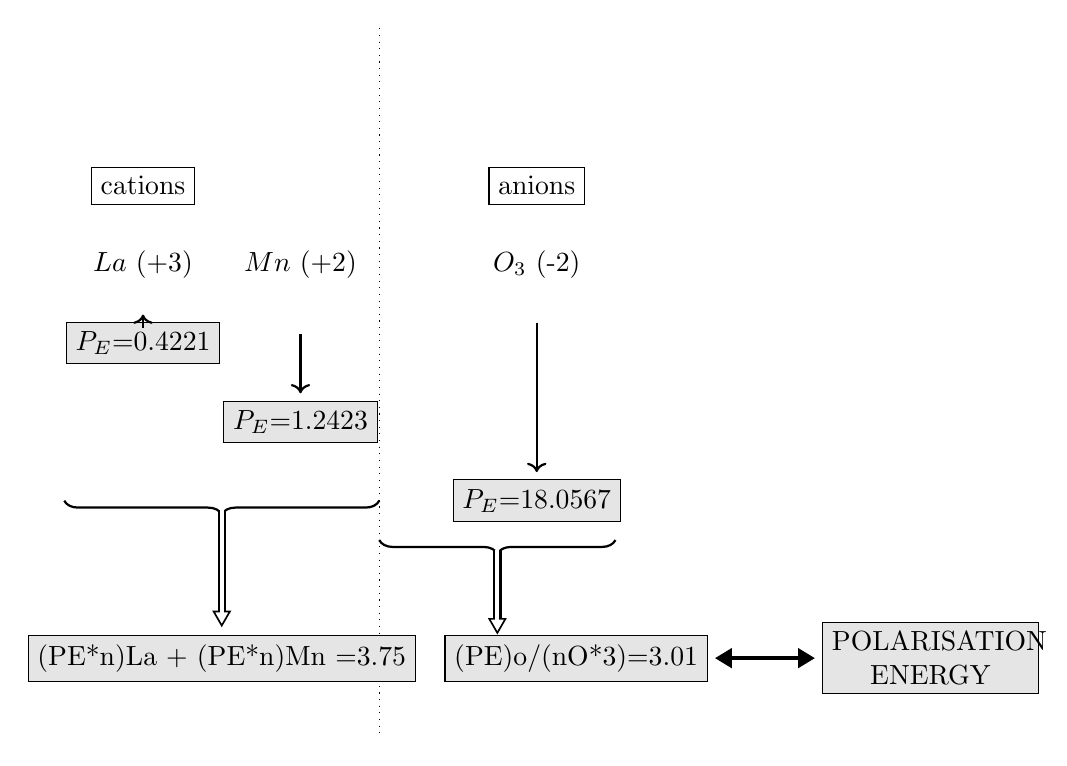
\begin{tikzpicture}
	%\draw node{cations};
	\node[rectangle,minimum size=0.01\textwidth,draw=black] (v1) at (0,0) {cations};
	\node[rectangle,draw=black] (v2) at (5,0) {anions};
	\node[circle] (E1) at (0,-1) {$La$ (+3)};
	\node[circle] (E2) at (2,-1) {$Mn$ (+2)};
	\node[circle] (E3) at (5,-1) {$O_3$ (-2)};
	\tikzstyle{edge}=[->,thick]
	\tikzstyle{arrow} = [ very thick, color=black, <->, >=Triangle]
	%\tikzstyle{line}=[draw,thick]
	%\tikzstyle{edge1}=[$\underbrace$,thick]
	\tikzstyle{block} = [draw,rectangle,fill=black!10,minimum size=0.005,outer sep=1mm,text centered,minimum height=2mm]
	%\node[rectangle](PE) at (0,-2) {$0.4221$};
	\node[block](PE1) at (0,-2) {$P_E$=0.4221};
	\draw[edge](E1)--(PE1);
	\node[block,minimum size=1mm](PE2) at (2,-3) {$P_E$=1.2423};
	\draw[edge](E2)--(PE2);
	\node[block](PE3) at (5,-4) {$P_E$=18.0567};
	\draw[edge](E3)--(PE3);
	\node[block,text width=2.5cm](F4) at (10,-6) { POLARISATION ENERGY };
	%\node[below=1cm](E1) {La};
	%\node[below=1cm
	%\node[circle,draw=black] (v1) at (0,0) {La};
	%\tikzstyle{vertex} = [square]
	%\node[vertex](v2)at(2,0){Mn};
	%\draw[edge1](PE1)--(PE2);
	\draw[decorate,thick,decoration={brace,amplitude=5pt,mirror}] 
	(-1,-4) -- 
	(3,-4){}; 
	\draw (1,-4pt) coordinate (t_k)  {};
	\node(B1) at (1,-4){};
	\node(B2) at (4.5,-4.5){};
	\draw[dotted](3,2)--(3,-7);
	\draw[decorate,thick,decoration={brace,amplitude=5pt,mirror}] 
	(3,-4.5) -- 
	(6,-4.5){};
	\node[block,minimum size=1mm](F1) at (1,-6) {(PE*n)La + (PE*n)Mn  =3.75};
	\node[block,right of=F1](F2) at (4.5,-6) {(PE)o/(nO*3)=3.01};
	\tikzstyle{vecArrow} = [thick, decoration={markings,mark=at position
		1 with {\arrow[semithick]{open triangle 60}}},
	double distance=1.4pt, shorten >= 5.5pt,
	preaction = {decorate},
	postaction = {draw,line width=1.4pt, white,shorten >= 4.5pt}]
	\draw[vecArrow] (B1) to (F1);
	\draw[vecArrow] (B2) to (4.5,-5.7);
	\draw[arrow] (F2.east) to (F4.west);
	%  \path{vecArrow}(F2)--(F4);
	%\framebox[0.5\textwidth][l]{n= (+3)     \hspace{1 cm}  (+2) \hspace{4 cm} (-2)} 
	%\framebox[0.5\textwidth][l]{La    \hspace{2 cm}  Mn \hspace{4 cm} $O_3$} 
	\end{tikzpicture}
	
}


%\resizebox{250pt}{20pt}{
%	\begin{tabular}{|c|c|c|c|c|c|}
		%	\caption{MAGNETIC PARAMETRS f-shell}
%		\hline
%		n & $f_m$ & $\mu^{"} = \dfrac{2 n}{\pi}$ & $\chi_{V(c.g.s)}= \dfrac{\mu^{"}}{4 \pi}$ & \small{$\chi_{A(c.g.s)}= V_M*N_A*(\chi_v)$} &\small{ $\mu_s =  2.828 (\sqrt{{\chi_A T}}) $ B.M} \\
%		\hline
%		1.6 & 2.54 GHz &  1.0192 & $1.53X10^{3}$ & $2.32 X 10^{-3} $ & 2.53 B.M \\
%		\hline
%		2.1 & 7.7 GHz  & 1.3377 & $2.69 X 10^{-2}$ & $4.08 X 10^{-2}$ & 9.8 B.M \\
%		\hline
%	\end{tabular}
%}




%	\begin{tabular*}{0.5pt}{|c|c|c|c|c|}
%	\hline
%	\caption{MAGNETIC PARAMETRS d-shell}
%	$\mu$ & $ \mu^{''}$ & $\delta$ & $ \chi_m = \mu -1 $ & \tiny{$ \mu_J = \dfrac{1}{\mu_B} \sqrt{\frac{\chi_m ( 3kT)}{n_l \mu_o}}$}\\
%	\hline
%	1.032 & 269 &  3.4 & 0.032 &9.4 \\ 
%	\hline
%	2.57  & 20.59 & 2.34 & 1.57 & 2.53 \\ 
%	\hline
%\end{tabular*}



\subsection{Selection Criteria}
Subsection text here.
\begin{enumerate}
	\item{Derived Radius values: The derived radius values can be used to conclude the cation and the anion required for the MA by matching their atomic radii to the derived values}
	\item {$P_o $ Parameter ,Based on the matching of the atomic radii , we can add the $P_o$ values such that $\sum {P_o}_{cations} = \sum {P_o}_{anion}$ }. Based on this , we can select multiple cations for the sample.
	\item{2.In case of mixed oxides , the mole fraction ratio of each cation or oxide compound can be derived as :-
		CALCULATION FOR THE MOLAR RATIO :-
		Depending on the ratio of the polarizability of the cation to anion , we can have the estimated molar fraction as
		\begin{equation}
		m = \frac{N_a X {r_a}^3}{N_c X {r_c}^3}
		\end{equation}
		
		Using the above derived values of the radius and the molar ratio calculation, we concluded for $Ga_2 O_3$
		with $m = 0.04$ }






	\item{In case of special crystal structures like pervoskite , spinel , fluorite , the radius ratio of the cation to anion has to be matched with the specified crystal requirement viz. }
\end{enumerate}



Subsubsection text here.


% An example of a floating figure using the graphicx package.
% Note that \label must occur AFTER (or within) \caption.
% For figures, \caption should occur after the \includegraphics.
% Note that IEEEtran v1.7 and later has special internal code that
% is designed to preserve the operation of \label within \caption
% even when the captionsoff option is in effect. However, because
% of issues like this, it may be the safest practice to put all your
% \label just after \caption rather than within \caption{}.
%
% Reminder: the "draftcls" or "draftclsnofoot", not "draft", class
% option should be used if it is desired that the figures are to be
% displayed while in draft mode.
%
%\begin{figure}[!t]
%\centering
%\includegraphics[width=2.5in]{myfigure}
% where an .eps filename suffix will be assumed under latex, 
% and a .pdf suffix will be assumed for pdflatex; or what has been declared
% via \DeclareGraphicsExtensions.
%\caption{Simulation Results}
%\label{fig_sim}
%\end{figure}

% Note that IEEE typically puts floats only at the top, even when this
% results in a large percentage of a column being occupied by floats.


% An example of a double column floating figure using two subfigures.
% (The subfig.sty package must be loaded for this to work.)
% The subfigure \label commands are set within each subfloat command, the
% \label for the overall figure must come after \caption.
% \hfil must be used as a separator to get equal spacing.
% The subfigure.sty package works much the same way, except \subfigure is
% used instead of \subfloat.
%
%\begin{figure*}[!t]
%\centerline{\subfloat[Case I]\includegraphics[width=2.5in]{subfigcase1}%
%\label{fig_first_case}}
%\hfil
%\subfloat[Case II]{\includegraphics[width=2.5in]{subfigcase2}%
%\label{fig_second_case}}}
%\caption{Simulation results}
%\label{fig_sim}
%\end{figure*}
%
% Note that often IEEE papers with subfigures do not employ subfigure
% captions (using the optional argument to \subfloat), but instead will
% reference/describe all of them (a), (b), etc., within the main caption.




% Note that IEEE does not put floats in the very first column - or typically
% anywhere on the first page for that matter. Also, in-text middle ("here")
% positioning is not used. Most IEEE journals use top floats exclusively.
% Note that, LaTeX2e, unlike IEEE journals, places footnotes above bottom
% floats. This can be corrected via the \fnbelowfloat command of the
% stfloats package.



\section{Conclusion}
The conclusion goes here.





% if have a single appendix:
%\appendix[Proof of the Zonklar Equations]
% or
%\appendix  % for no appendix heading
% do not use \section anymore after \appendix, only \section*
% is possibly needed

% use appendices with more than one appendix
% then use \section to start each appendix
% you must declare a \section before using any
% \subsection or using \label (\appendices by itself
% starts a section numbered zero.)
%


%\appendices
%\section{Proof of the First Zonklar Equation}
%Appendix one text goes here.

% you can choose not to have a title for an appendix
% if you want by leaving the argument blank
%\section{}
%Appendix two text goes here.


% use section* for acknowledgement
\section*{Acknowledgment}


The authors would like to thank...


% Can use something like this to put references on a page
% by themselves when using endfloat and the captionsoff option.
\ifCLASSOPTIONcaptionsoff
\newpage
\fi



% trigger a \newpage just before the given reference
% number - used to balance the columns on the last page
% adjust value as needed - may need to be readjusted if
% the document is modified later
%\IEEEtriggeratref{8}
% The "triggered" command can be changed if desired:
%\IEEEtriggercmd{\enlargethispage{-5in}}

% references section

% can use a bibliography generated by BibTeX as a .bbl file
% BibTeX documentation can be easily obtained at:
% http://www.ctan.org/tex-archive/biblio/bibtex/contrib/doc/
% The IEEEtran BibTeX style support page is at:
% http://www.michaelshell.org/tex/ieeetran/bibtex/
\bibliographystyle{IEEEtran}
% argument is your BibTeX string definitions and bibliography database(s)
\bibliography{References}
%
% <OR> manually copy in the resultant .bbl file
% set second argument of \begin to the number of references
% (used to reserve space for the reference number labels box)
%\begin{thebibliography}{1}

%\bibitem{IEEEhowto:kopka}
%H.~Kopka and P.~W. Daly, \emph{A Guide to \LaTeX}, 3rd~ed.\hskip 1em plus
% 0.5em minus 0.4em\relax Harlow, England: Addison-Wesley, 1999.

%\end{thebibliography}

% biography section
% 
% If you have an EPS/PDF photo (graphicx package needed) extra braces are
% needed around the contents of the optional argument to biography to prevent
% the LaTeX parser from getting confused when it sees the complicated
% \includegraphics command within an optional argument. (You could create
% your own custom macro containing the \includegraphics command to make things
% simpler here.)
%\begin{biography}[{\includegraphics[width=1in,height=1.25in,clip,keepaspectratio]{mshell}}]{Michael Shell}
% or if you just want to reserve a space for a photo:

%\begin{IEEEbiography}{Michael Shell}
%Biography text here.
%\end{IEEEbiography}

% if you will not have a photo at all:
%\begin{IEEEbiographynophoto}{John Doe}
%Biography text here.
%\end{IEEEbiographynophoto}

% insert where needed to balance the two columns on the last page with
% biographies
%\newpage

%\begin{IEEEbiographynophoto}{Jane Doe}
%Biography text here.
%\end{IEEEbiographynophoto}

% You can push biographies down or up by placing
% a \vfill before or after them. The appropriate
% use of \vfill depends on what kind of text is
% on the last page and whether or not the columns
% are being equalized.

%\vfill

% Can be used to pull up biographies so that the bottom of the last one
% is flush with the other column.
%\enlargethispage{-5in}



% that's all folks
\end{multicols}
\end{document}
